\begin{figure}[h]
    \centering
    \begin{subfigure}[t]{0.64\textwidth}
        \centering
        \includegraphics[width=\linewidth]{images/osc/osc_circuit.png}
        \caption{Oscillator+Matching Network Topology}
        \label{fig:osc_and_match}
    \end{subfigure}
    \hfill
    \begin{subfigure}[t]{0.35\textwidth}
        \centering
        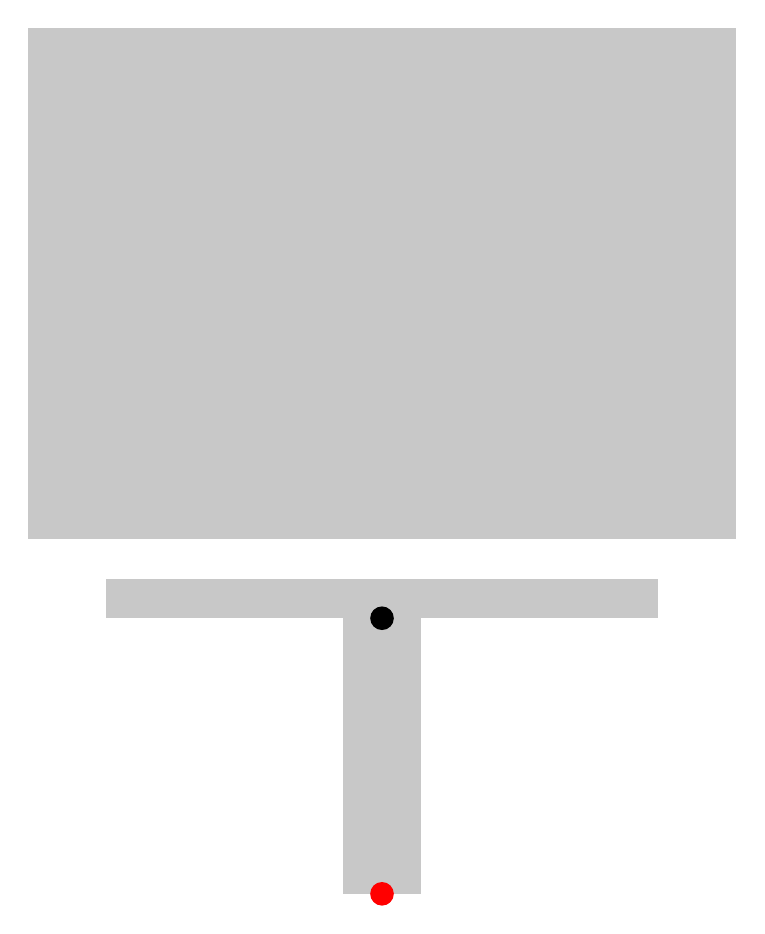
\begin{tikzpicture}
            \definecolor{mycolor}{RGB}{200,200,200}
            % Draw a grey rectangle without borders
            \fill[mycolor] (0,0) rectangle (9,6.5);
            \fill[mycolor] (1, -1) rectangle (8, -0.5);
            \fill[mycolor] (4, -4.5) rectangle (5, -1);
            \fill (4.5, -1) circle (0.15);
            \fill[red] (4.5, -4.5) circle (0.15);
        \end{tikzpicture}
        \caption{Wideband Patch Antenna}
        \label{fig:patch-antenna}
    \end{subfigure}
    \caption{Design and Topology of primary components}
    \label{fig:combined}
\end{figure}

% ================================================ OSC =====================================

\textbf{Oscillator:}
The Colpitts oscillator topology is ideal for a\(3.5[GHz]\) oscillator due to its excellent frequency stability, making it suitable for precise frequency control in communication systems. Its easy tuning capability allows for straightforward frequency adjustments by changing capacitors and inductors. Additionally, Colpitts oscillators typically exhibit low phase noise, crucial for maintaining signal integrity and reducing interference in RF applications. The topology’s simplicity and cost-effectiveness further enhance its practicality, making it a preferred choice for stable and efficient\(3.5[GHz]\) oscillator designs. To ensure reliable functioning of the oscillator, startup conditions obtained using small-signal analysis were withheld~\cite{Johnson1986ACO}. The SSM gave us
\[\frac{v_{out}}{i_{in}} = \frac{r_\pi L_p R_L(s^2C + sg_m)}{r_\pi C^2L_p R_L s^3  +(- r\pi C L_p R_L g_m + 2r_\pi CL_p + CL_pR_L)s^2 + (2r_\pi CR_L + L_p)s + R_L}\]
We attained conditions: \(\displaystyle \omega_0 \approx \sqrt{\frac{1}{\displaystyle L\frac{C_1 C_2}{C_1+C_2}}}\)\footnote{Assuming \(r_\pi (C_1+C_2)R_L >> L_p\)} and \(\displaystyle R_L (g_m) - \frac{R_L}{(r_\pi)} - 2 > 0\)

\begin{comment}
After deciding on the Colpitts topology, startup conditions were derived from the following small signal-based equation: \(\displaystyle i_{in} = -\frac{v_{\pi}}{r_{\pi}} - sC(v_{out} + 2v_{\pi})\) and \(\displaystyle 0 = g_mv_{\pi} + sC(v_{out} + v_{\pi}) + \frac{v_{out}}{sL_p} + \frac{v_{out}}{R_L}\).

We attained the approximation for operating frequency and startup condition: \(\displaystyle \omega_0 \approx \sqrt{\frac{1}{L\frac{C_1 C_2}{C_1+C_2}}}\) and \(\displaystyle R_L g_m - \frac{R_L}{r_\pi} - 2 > 0\).\par
\end{comment}

